\chapter{What is open, and the plan to close it}\label{ch:open}

\section*{How to read this list}
Figure~\ref{fig:open_items} counts the items below by group, by who can settle them, and by the Part they come from.
\begin{figure}[htbp]\centering
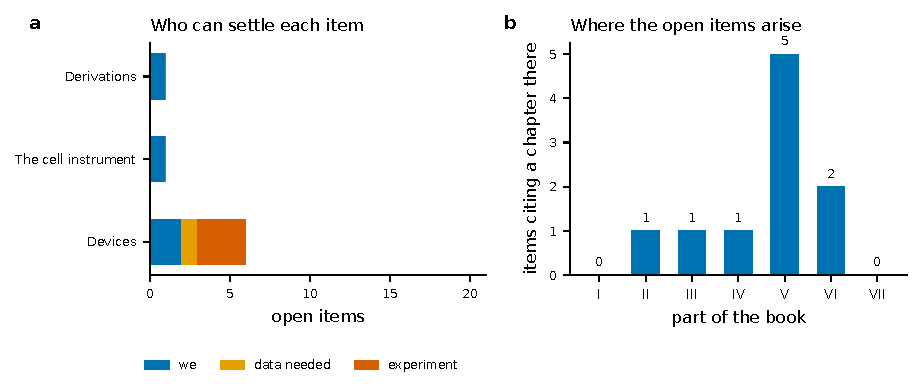
\includegraphics[width=\textwidth]{figures/part7/fig_open_items.pdf}
\caption{(a) The open items of this chapter by group and by who can settle them. (b) The Part in which each item's cited chapter lies. Counted from the tables of this chapter by the figure script. \calc}\label{fig:open_items}
\end{figure}
Every item below is stated as open somewhere in the book. Each is given with where it arises, what would settle it, and who can settle it:
\textbf{we} (a calculation, or data already public and in hand), \textbf{data due} (a survey or measurement already scheduled), or
\textbf{experiment} (a measurement that needs a laboratory we do not have, for which the book states the design). Items are in order of
consequence within each group.

\section{Derivations}
{\small\begin{longtable}{@{}>{\raggedright\arraybackslash}p{0.33\textwidth}>{\raggedright\arraybackslash}p{0.43\textwidth}>{\raggedright\arraybackslash}p{0.16\textwidth}@{}}
\toprule
open item & what settles it & who \\\midrule\endhead
\textbf{D1. The cell's floor from the law alone.} The chip and qubit floors follow from $\kB T$ at the temperature the record sees; the
 cell's floor height is measured, not yet derived (Chapters~\ref{ch:iama},~\ref{ch:saturation}).
 & The steady-state copy error of a site under a writing process of finite discrimination, with the copying and removal rates
   measured for neutrophils, should give $\varepsilon_0$ and so $E_{\rm hold}=3.41\,\kB T$. For processors, the constants of the coherence
   optimum measured on one material.
 & we \\\cmidrule[0.2pt]{1-3}
\textbf{D2. The architecture position $P$.} The neutrophil's $P=1.099$ is measured from three donors (Chapter~\ref{ch:iama}).
 & A rule for $P$ from the cell's own maintenance rates, tested on a second cell type before its $P$ is measured. & we \\\cmidrule[0.2pt]{1-3}
\textbf{D3. The electron-mass prefactor.} $(2\pi)^{3/10}$ was found by search (Chapter~\ref{ch:electronmass}).
 & A derivation, or a replacement, stated with the sector of $H_0$ it uses. & we \\\cmidrule[0.2pt]{1-3}
\textbf{D4. The $3/16$ and the $2/\pi$.} $\Omega_b/\Omega_m=(3/16)\sqrt{\Omega_\Lambda}$ holds at $0.7\sigma$ and the $2/\pi$ of the
 vacuum estimate is not derived (Chapter~\ref{ch:lambda}).
 & One calculation from the de Sitter causal structure that fixes the geometric factor, the temperature factor and the baryon fraction together. & we \\\cmidrule[0.2pt]{1-3}
\textbf{D5. Three generations, and the Koide offset.} Positivity allows at most three; $n=2$ is allowed for $\delta\ne0$; $\delta=0.22227$ is
 measured, not derived (Chapter~\ref{ch:koide}). & A principle that excludes $n=2$ and fixes $\delta$. & we \\\cmidrule[0.2pt]{1-3}
\textbf{D6. The two exponents.} The cosmology takes $7/2$ and the electron mass $5/2$ (Chapter~\ref{ch:nonlocal}).
 & Show whether one follows from the other, or state that they are unrelated. & we \\\cmidrule[0.2pt]{1-3}
\textbf{D7. The informational $w(a)$.} $w_{\rm info}=-1-1/(3a)$ on the matter ruler is stated, not compared (Chapter~\ref{ch:darkenergy}).
 & A full matter-ruler $w(a)$ and its comparison with the DESI distance-only and growth-only fits (prediction C14). & we \\\cmidrule[0.2pt]{1-3}
\textbf{D8. The cluster test's form.} The lensing-to-hydrostatic ratio $1/\mu(z)$ holds only in the Level~1 form (prediction C17).
 & Settle which form of the coupling the cluster masses see, then rerun the forecast. & we \\\cmidrule[0.2pt]{1-3}
\textbf{D9. The decoherence ramp.} The rate integral gives an exponential; the sigmoidal ramp used for decoherence, erasure and Bell
 tests is assumed (Chapters~\ref{ch:gravdec},~\ref{ch:measurement}). & Derive the time dependence, or replace the ramp everywhere by the exponential. & we \\\cmidrule[0.2pt]{1-3}
\textbf{D10. Two sectors, one ladder.} Why distance-ladder supernovae, measured in light, read the matter-sector rate (Chapter~\ref{ch:dual}).
 & A derivation of which ruler a calibrated distance indicator inherits. & we \\\cmidrule[0.2pt]{1-3}
\textbf{D11. Measurement and erasure.} Where the criterion $Q\ge Q_L$ sits relative to Bennett's result that only erasure has a minimum cost
 (Chapter~\ref{ch:measurement}). & Restate the criterion as the condition for irreversibility at absorption and check it against cavity experiments. & we \\\cmidrule[0.2pt]{1-3}
\textbf{D12. The record history.} The first law fixes the entropy history the record term needs: $dS_{\rm info}/d\ln a=\beta_mS_{\rm geo}$
 today, $5.2\times10^{121}$ bits per e-fold (Appendix~\ref{app:der:record}).
 & Count the bits written by structure formation per e-fold from measured halo statistics and compare. & we \\\cmidrule[0.2pt]{1-3}
\textbf{D13. The exponential.} The first law is linear in $S_{\rm info}$; $\rho_{\rm info}\propto E(a)$ rests on the record constraint, or on an
 exponentiation postulate with an unfixed scale $S_0$ (Appendix~\ref{app:der:routes}).
 & Derive the constraint $\dot\rho_{\rm info}=\rho_{\rm info}H/a$, or the exponentiation and its scale, from the horizon accounting. & we \\\cmidrule[0.2pt]{1-3}
\textbf{D14. The amplitude of the exponent.} The scaling fixes the shape $-1/a$; the coefficient of $1/a$ is the normalization of $S_{\rm info}$
 (Appendix~\ref{app:der:exponent}). & Fix the amplitude from the absolute record rate, not from the fit. & we \\\cmidrule[0.2pt]{1-3}
\textbf{D15. A covariant action.} $\dot\varphi=H/a$ is defined on the FRW minisuperspace only, and $\delta\varphi=0$ is a property of the reduced
 action (Appendix~\ref{app:der:variational}). & Write the constraint covariantly (for example through the expansion of a preferred matter flow) and
 derive the perturbation equations from it. & we \\\cmidrule[0.2pt]{1-3}
\textbf{D16. The sector split.} The first law and the action both modify the background; the Level~2b chains exclude that (Chapter~\ref{ch:level2}).
 & Derive why the record term enters the matter perturbations only. & we \\\cmidrule[0.2pt]{1-3}
\textbf{D17. Which growth equation.} The $G_{\rm eff}$, friction and full forms give $-0.78$, $-0.67$ and $-1.87\,\%$ in $D$ today
 (Appendix~\ref{app:der:growth}). & Derive the form from the record term, then use one form for every growth number. & we \\\cmidrule[0.2pt]{1-3}
\textbf{D18. The running exponent.} Halo statistics give $n_{\rm eff}$ from about $5.5$ ($z=9$) to $2$ ($z=1$), equal to $7/2$ at $z\approx3$--$4$
 (Chapter~\ref{ch:quantumrecords}). & Include merger heating and the $\rho_{\rm crit}(z)$ scaling of the halo kinetic energy; state whether the running
 survives. & we \\\cmidrule[0.2pt]{1-3}
\textbf{D19. The coupling over the ensemble of halos.} $\beta_m=\Omega_m/2$ applies an equilibrium theorem to non-equilibrium structure, with the
 present-day $\Omega_m$ (Appendix~\ref{app:der:coupling}). & A cosmological energy partition over the ensemble of halos and its time dependence;
 growth data at Euclid precision. & we, data needed \\\cmidrule[0.2pt]{1-3}
\textbf{D20. The superposition boundary.} The capacity $k_BT/E_G$ and the rate $E_G^2/(\hbar k_BT\ln2)$ behind $\tau_{\rm IAM}$ are postulated
 (Appendix~\ref{app:der:quantum}). & Derive both at the boundary of a massive superposition, as the horizon accounting does for $E(a)$. & we \\
\bottomrule
\end{longtable}}

\section{The cell instrument}
{\small\begin{longtable}{@{}>{\raggedright\arraybackslash}p{0.33\textwidth}>{\raggedright\arraybackslash}p{0.43\textwidth}>{\raggedright\arraybackslash}p{0.16\textwidth}@{}}
\toprule
open item & what settles it & who \\\midrule\endhead
\textbf{I1. Commissioning neutrophils in whole blood.} The chain reads purified neutrophils and constructed mixtures; it has not been
 commissioned on real whole blood. & Pre-registered tests through the chain, end to end: repeat draws and technical replicates, infection, autoimmune
 disease, myeloid disease, pre-diagnosis blood; the public sets are being collected now (Appendix~\ref{appendices:app:repro}). & we \\\cmidrule[0.2pt]{1-3}
\textbf{I2. Breach and the cancer region on this gauge.} Not placed (Chapter~\ref{ch:gauge}).
 & Per-person data on the current scale: tumor--normal pairs, the DNMT1-inhibitor series, blood cancers. & we \\\cmidrule[0.2pt]{1-3}
\textbf{I3. The Met-A floor.} $H_{\min}$ on the Met-A scale is not defined (Chapter~\ref{ch:gauge}). & Relate the array reading to the
 molecule-level floor through matched array and sequencing data from the same specimens. & we, data needed \\\cmidrule[0.2pt]{1-3}
\textbf{I4. Repeatability.} The smallest change between two draws of one person that the instrument can call is not yet measured (Chapter~\ref{ch:serial}). & Same-chip technical replicates through the
 chain's own Stage~1. & we \\\cmidrule[0.2pt]{1-3}
\textbf{I5. Past the entropy ceiling.} Met-A is monotone only while methylated sites stay above $\beta=\tfrac12$ (Chapter~\ref{ch:meta}).
 & Print the mean $\beta$ beside Met-A and flag readings past half-loss; a dose series in the range where $\beta$ stays above 0.5. & we \\\cmidrule[0.2pt]{1-3}
\textbf{I6. Below 1.} What a reading below 1 means for a cell (senescence is the candidate) has not been measured (Chapter~\ref{ch:floorbreach}).
 & Purified senescent and quiescent cells read against their own healthy reference. & we, data needed \\\cmidrule[0.2pt]{1-3}
\textbf{I7. The IAM-A C-score.} Defined, not built (Chapter~\ref{ch:cscore}). & Build it from per-region copy error on molecules; test on the
 tumor pairs and the DNMT1 series. & we \\\cmidrule[0.2pt]{1-3}
\textbf{I8. A physical zero for each laboratory.} The two routes are recorded and not started (Chapter~\ref{ch:instrument}). & A response model from
 the control probes, or a reference material of known methylation run through each laboratory. & we, experiment \\\cmidrule[0.2pt]{1-3}
\textbf{I9. Eosinophil and neutrophil fractions} outside the bar on known mixtures (Chapter~\ref{ch:separation}). & Find the source of the shortfall
 in the atlas profiles or the solver. & we \\\cmidrule[0.2pt]{1-3}
\textbf{I10. Identity sites for the next cell types.} On atlas v2, held-out transfer of identity sites reached 87.7\,\% and 73.1\,\% against a bar of 95\,\% (Chapter~\ref{ch:atlas}). & More purified
 samples per cell on one platform, to separate site-choice noise from donor spread. & we \\\cmidrule[0.2pt]{1-3}
\textbf{I11. Whole-array sky maps} need a sex mask: one female reference array lights chrX against five male ones (Chapter~\ref{ch:skytools}). & Redraw the six-array sky with chrX and chrY masked, and with sex-matched references. & we \\\cmidrule[0.2pt]{1-3}
\textbf{I12. Conversion failure on the unmethylated channel} in the IMR90 cultures (Chapter~\ref{ch:gauge}). & Read conversion from the
 non-CpG cytosines of the same libraries. & we \\\cmidrule[0.2pt]{1-3}
\textbf{I13. Temperature.} Whether the floor moves with temperature at fixed holding energy (Chapter~\ref{ch:temperature}). & One species, one cell
 type, one pipeline at two recorded temperatures, with molecular identifiers and a per-library known-pattern control. & we \\\cmidrule[0.2pt]{1-3}
\textbf{I14. More cell types,} one at a time, each commissioned before it is read. & Each cell's own healthy reference on purified cells. & we \\
\bottomrule
\end{longtable}}

\section{Devices}
{\small\begin{longtable}{@{}>{\raggedright\arraybackslash}p{0.33\textwidth}>{\raggedright\arraybackslash}p{0.43\textwidth}>{\raggedright\arraybackslash}p{0.16\textwidth}@{}}
\toprule
open item & what settles it & who \\\midrule\endhead
\textbf{Q1. The quasiparticle single-device check} $x_{qp}\tau_{\rm TLS}n_{cp}V/(N\tau_{qp})=2$ (Chapter~\ref{ch:xqp}). & One device with all five quantities
 measured. & experiment \\
\textbf{Q2. The $T_1$ ceiling} of about 0.24\,ms for an aluminum transmon at $x_{qp}\approx10^{-7}$ (prediction X3). & Compare with published
 record lifetimes of isolated Al-electrode transmons. & we \\
\textbf{Q3. Temperature of a qubit.} The thermal floor is set by the qubit's own effective temperature, which is typically higher than the
 refrigerator plate (Chapters~\ref{ch:thermaln},~\ref{ch:qplatforms}). & Collect published sweeps that report the effective temperature with $T_1$,
 gate time and two-qubit error on one device. & we \\
\textbf{Q4. The ion gate's floor.} The ion's hyperfine record is not thermalized; its gate runs through the motional bus, whose floor is set by
 the heating rate and the gate time (Chapters~\ref{ch:ascoreqc},~\ref{ch:qplatforms}). & Per-mode heating rate, $\bar n$ at the start of the gate
 and the gate time, measured on one apparatus. & experiment \\
\textbf{Q5. The drive optima.} The forms $A/P+BP$ for laser-gate ions and $a/\Omega+b\Omega^2$ for Rydberg gates are models whose
 constants are unmeasured (Chapters~\ref{ch:walls},~\ref{ch:qplatforms}). & The two-qubit error against drive on one apparatus at fixed heating
 or fixed environment temperature. & experiment \\
\textbf{Q6. A per-block chip reading.} The chip figure averages over idle transistors (Chapter~\ref{ch:cmos}). & A design's own power and
 activity data per block. & data needed \\
\bottomrule
\end{longtable}}

\section{Measurements that would settle the most}
Figure~\ref{fig:open_map} shows where in the book the open problems are labeled.
\begin{figure}[htbp]\centering
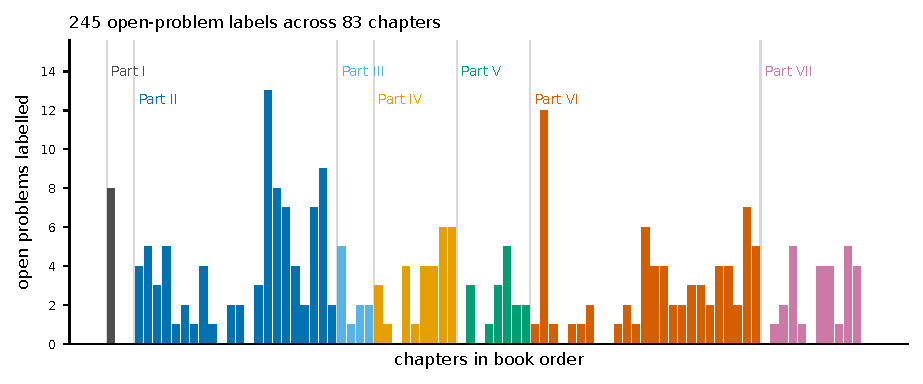
\includegraphics[width=\textwidth]{figures/part7/fig_open_map.pdf}
\caption{Open-problem labels per chapter, in book order, colored by Part, counted from the chapter sources by the figure script. \calc}\label{fig:open_map}
\end{figure}
In order: Euclid's $\mu_0$ and $\Sigma$ (mid-2027 and final survey); percent redshift-space distortions in redshift bins (DESI full survey);
a growth-only fit with the IAM template; a siren sample precise enough to separate 67.16 from 72.26; a levitated-sphere coherence time at three
internal temperatures; one superconducting device with $x_{qp}$, $\tau_{\rm TLS}$, $\tau_{qp}$, $N$ and $V$ measured together; and, for the cell,
the commissioning tests of item I1. Three chain runs need no new data: the free-$\mu_0$ chains with a wider prior, to show where the
posterior turns over (Chapter~\ref{ch:latetime}); the Level~2 growth run repeated with $f\sigma_8$ computed as $d\sigma_8/d\ln a$; and the
Level~1 fixed-$\mu_0$ chains with the exact coupling $\mu=H^2/(H^2+\beta_mE(a)H_0^2)$ in place of the MGCAMB form. \openprob{} When Euclid's
data are public, both chain levels are rerun with them, with the wide prior from the start. The predictions they test, with their falsifiers,
are in Chapter~\ref{ch:predictions}.

\section{The decisive tests}
IAM makes definite statements, and each of these would test it directly. Every one is within reach of experiments running now or planned.
\begin{enumerate}
\item Euclid measures $\mu_0$ consistent with 0 and excluding $-0.136$, or finds $\Sigma\ne1$.
\item The $f\sigma_8$ deficit is absent at survey precision, or is a constant factor rather than the ramp of prediction C3.
\item Standard sirens, with enough events, exclude 72.26 for the matter flow.
\item A levitated body's coherence time is independent of, or falls with, its internal temperature where $\tau_{\rm IAM}$ is accessible.
\item A chip switches an irreversible bit for less than $\kB T_j\ln2$.
\item Purified healthy cells of a commissioned type, from donors not used in its reference, read systematically outside Normal on their own
      identity sites, with composition verified.
\item Two technical replicates of the same DNA on the same chip differ by more than the width of Normal.
\item A known loss of maintenance fidelity, at a dose that keeps methylated sites above $\beta=\tfrac12$, is not read on the methylated channel.
\end{enumerate}

Every test on this list can be run by someone working in that field today. Each one is a clean way to find out where the framework stands, and that is the best reason to run it.
